\documentclass[11pt]{article}

\usepackage[utf8]{inputenc}
\usepackage[T1]{fontenc}
\usepackage[margin=1in]{geometry}
\usepackage{algorithm}
\usepackage{algpseudocode}
\usepackage{tikz}
\usepackage{amsmath, amssymb}
\usepackage{float}
\usetikzlibrary{trees}

\bibliographystyle{plain}


\title{TODO Add a name}
\author{Kevin Chen}
\date{\today}

\begin{document}

\maketitle

\section{Introduction}

TODO insert introduction

\section{Symbolic Execution}

Symbolic execution is a way of executing a program abstractly, such that on abstract execution covers multiple possible inputs of the program that share a particular execution path through the code \cite{aldrich2018symbolic}. Each input of symbolicly executed code is represented as a symbol rather than assigning it a concrete value. When the value is referenced such as for an if statement, the execution path branches, where one path the symbolic value is evaluated as true while the other path the symboilic value is evaluated as false.

One of the key uses for symbolic execution is in testing. Most unit tests, require the programmer to hardcode in values to test, resulting in various unit tests to cover all branches the code can tranverse. On the other hand, a symbolic execution would execute simutaneously on a family of inputs. Consider the following example:

\begin{algorithm}
    \caption{Algorithm 1}
    \label{alg:simple-example}
    \begin{algorithmic}[1]
    \Require $x, y \in \mathbb{Z}$
    \State $a \gets x + y$
    \If{$a \bmod 2 = 0$}
        \State \Return error ``$a$ is even''
    \Else
        \State \Return $a$
    \EndIf
    \end{algorithmic}
\end{algorithm}
    
With a glance, we can see that using any combination of numbers such that their sum results in an even number will result in an error. There is no way to cover all cases of failure using unit tests, as there are an infinite number of way which we can stumble onto this error.

Instead of testing with unit tests such as $x=1, y=1$, symbolic execution represents the inputs as symbols $x=x_0, y= y_0$. Whenever, the symbols are required to return a value, such as in a branch, symbolic execution splits into two executions, with each execution recording the branching condition in its execution path. Consider a symbolic execution of the algorithm above. We start with representing each input symbolicly:

\begin{figure}[H]
    \centering
    \begin{tabular}{|c|c|c|}
        \hline
        line & Path Condition & Translation \\
        \hline
        0 & true & $x\to x_0, y\to y_0$ \\
        1 & true & $x\to x_0, y\to y_0, a\to x_0+y_0$ \\
        2 & $(x_0 + y_0) \bmod 2 = 0$ & $x\to x_0, y\to y_0, a\to x_0+y_0$ \\
        2 & $\neg((x_0 + y_0) \bmod 2 = 0)$ & $x\to x_0, y\to y_0, a\to x_0+y_0$ \\
        3 & $(x_0 + y_0) \bmod 2 = 0$ & Error \\
        5 & $\neg((x_0 + y_0) \bmod 2 = 0)$ & Return $x_0 + y_0$ \\
        \hline
    \end{tabular}
    \caption{Symbolic execution trace showing path conditions and variable translations}
    \label{fig:symbolic-trace}
\end{figure}

In this example, we see that the inputs values start symbolic as symbols which has no concrete value. Following the execution, we translate every instance of $x$ with $x_0$ with the same case for $y$. Where it gets interesting is when the the execution has a branching path. In the $\textbf{if}$ statement, the value of a is required to be assigned a value, which breaks the symbolic abstraction. Instead, the symbolic execution branches into two different executions, each of which assuming a different condition to satisfy the branching statement. Below we can visualize the different execution paths the execution takes via a simple tree (see Figure~\ref{fig:execution-tree}):

\begin{figure}[H]
    \centering
    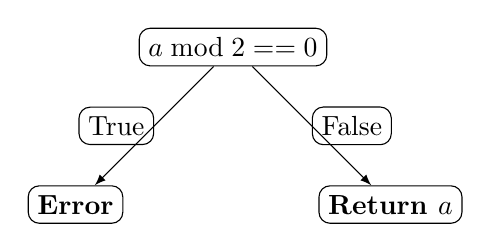
\begin{tikzpicture}[
        level distance=2cm,
        sibling distance=4cm,
        every node/.style={draw, rounded corners, align=center},
        edge from parent/.style={draw, -latex}
      ]
      
      \node {$a \bmod 2 == 0$}
          child { node {\textbf{Error}}
              edge from parent node[left] {True}
          }
          child { node {\textbf{Return $a$}}
              edge from parent node[right] {False}
          };
      
      \end{tikzpicture}
    \caption{Execution tree showing the branching paths in symbolic execution}
    \label{fig:execution-tree}
\end{figure}

In each paths, we accumulate the different path conditions until we either reach the end (return statement) or a failure (error). In this case, we find that there exists a set of inputs (when $x_0+y_0 \bmod 2 = 0$), which causes an error. Now imagine a different example; using the same coding example, but with a twist. Prior to running this program with symbolic execution, one can add constraints to the path. Below, an example where we start with a given constraint that $x_0+y_0=1$:

\begin{figure}[H]
    \centering
    \begin{tabular}{|c|c|c|}
        \hline
        line & Path Condition & Translation \\
        \hline
        0 & $x_0+y_0=1$ & $x\to x_0, y\to y_0$ \\
        1 & $x_0+y_0=1$ & $x\to x_0, y\to y_0, a\to x_0+y_0$ \\
        2 & $\neg((x_0 + y_0) \bmod 2 = 0)$ & $x\to x_0, y\to y_0, a\to x_0+y_0$ \\
        2 &  $x_0+y_0=1 \land (x_0 + y_0) \bmod 2 = 0$ & $x\to x_0, y\to y_0, a\to x_0+y_0$ \\
        3 & False & Error \\
        5 & $\neg((x_0 + y_0) \bmod 2 = 0)$ & Return $x_0 + y_0$ \\
        \hline
    \end{tabular}
    \caption{Modified version of execution with existing constraints}
    \label{fig:symbolic-trace-with-constraint}
\end{figure}

With the constraint, the path condition which leads to the error is contradictory. This illustrates that the path is impossible. With this constraint, we see that no path leads to any errors. In industry, programmers, can create tests with given preconditions (constraints) and run until the program terminates. Instead of throwing an error, we can use assertion statements as post-conditions. If it terminates without an error, the program is robust across all set of inputs. Otherwise, a symbolicly executed program will return a concrete set of conditions which will give an error or violate a post-condtiion.

\subsection{While loops}

To represent a while loop in symbolic execution, we unroll it into a recursive function with no loops. Take the following code for instance:

\begin{algorithm}
    \caption{Count Number of 1's in a Bit Vector}
    \label{alg:count-ones-while}
    \begin{algorithmic}[1]
    \Require $v$ is a bit vector of length $n$
    \State $count \gets 0$
    \State $i \gets 0$
    \While{$i < n$}
        \If{$v[i] == 1$}
            \State $count \gets count + 1$
        \EndIf
        \State $i \gets i + 1$
    \EndWhile
    \State \Return $count$
    \end{algorithmic}
\end{algorithm}

We can rewrite it as a recursive function: 

\begin{algorithm}
    \caption{Recursively Count Number of 1's in a Bit Vector}
    \label{alg:recursive-count-ones}
    \begin{algorithmic}[1]
    \Require $v$ is a bit vector of length $n$
    \Function{count\_ones}{$v, i, n$}
        \If{$i == n$}
            \State \Return $0$
        \ElsIf{$v[i] == 1$}
            \State \Return $1 +$ \Call{count\_ones}{$v, i+1, n$}
        \Else
            \State \Return \Call{count\_ones}{$v, i+1, n$}
        \EndIf
    \EndFunction
    \State \Return \Call{count\_ones}{$v, 0, n$}
    \end{algorithmic}
\end{algorithm}

Now that we have rewritten the while loop as if statements, we simply create a new branch for every if statement. In practice, this may lead to state explosion, resulting in thousands of branches in a just a few iterations. Programmers either set a recursion limit, terminating the branch which gets stuck, or find a different way to represent the while loop, using the loop invariant. Below is a tree of the branching paths created from a symbolic execution of Algorithm~\ref{alg:recursive-count-ones}. 

\begin{figure}[H]
    \centering
    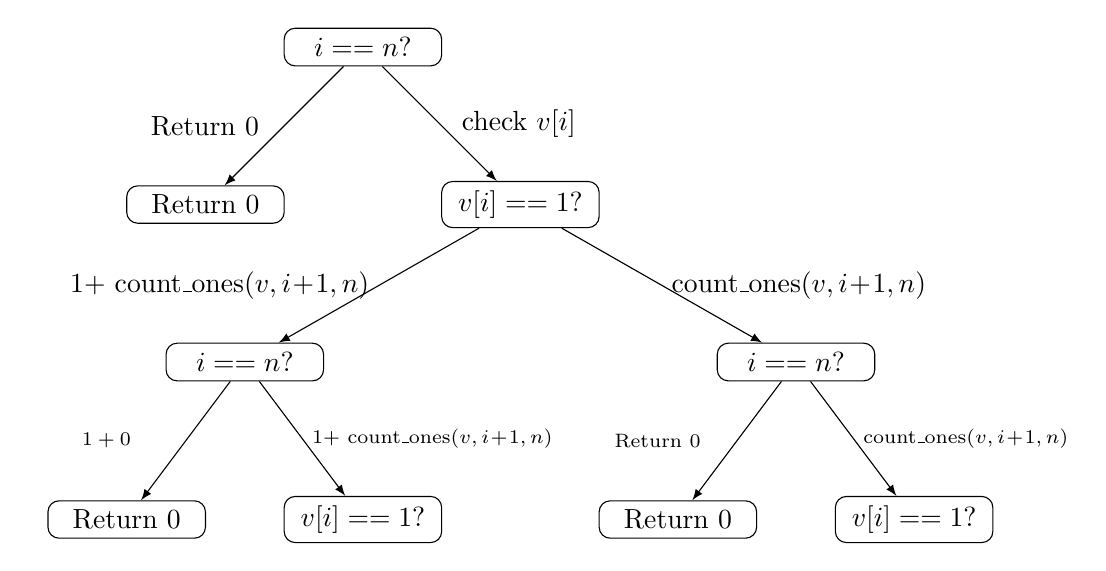
\begin{tikzpicture}[
        level 1/.style={sibling distance=4cm, level distance=2cm},
        level 2/.style={sibling distance=7cm, level distance=2cm},
        level 3/.style={sibling distance=3cm, level distance=2cm},
        every node/.style={draw, rounded corners, align=center, minimum width=2cm},
        edge from parent/.style={draw, -latex}
      ]
      
      \node {$i == n$?}
          child { node {Return 0}
              edge from parent node[left, draw=none] {Return 0}
          }
          child { node {$v[i] == 1$?}
              child { node {$i == n$?}
                  child { node {Return 0}
                      edge from parent node[left, draw=none, font=\scriptsize] {$1 + 0$}
                  }
                  child { node {$v[i] == 1$?}
                      edge from parent node[right, draw=none, font=\scriptsize] {$1 +$ count\_ones($v, i\!+\!1, n$)}
                  }
                  edge from parent node[left, draw=none] {$1 +$ count\_ones($v, i\!+\!1, n$)}
              }
              child { node {$i == n$?}
                  child { node {Return 0}
                      edge from parent node[left, draw=none, font=\scriptsize] {Return 0}
                  }
                  child { node {$v[i] == 1$?}
                      edge from parent node[right, draw=none, font=\scriptsize] {count\_ones($v, i\!+\!1, n$)}
                  }
                  edge from parent node[right, draw=none] {count\_ones($v, i\!+\!1, n$)}
              }
              edge from parent node[right, draw=none] {check $v[i]$}
          };
      
      \end{tikzpicture}
    \caption{Symbolic execution tree for the recursive count\_ones algorithm showing branching at each condition}
    \label{fig:recursive-execution-tree}
\end{figure}

\section{Hardware Language}


\section{Patronus}

\subsection{Expressions}

Patronus\cite{cucapra2024patronus} represents expressions under the class \textit{Expr} and $\textit{ExprRef}$. Each expression is an object which contains the type of expression and a list of \textit{ExprRef} to other expressions. For example, the expression $if (x==4, y+=3, z+=4)$ can be represented as $ite(\textit{ExprRef}[1], \textit{ExprRef}[2], \textit{ExprRef}[3])$. The expressions are stored all in an Context.

\section{Implementation}

\subsection{Symbolic Execution}

One of the key challenges of implementing symbolic execution is being able to distinguish whether or not a path is feasible or not. Consider the execution from Figure~\ref{fig:symbolic-trace-with-constraint} row 3. The question are we suppose to tell that this path represents is infeasible?

As always in computer science, one of the best ways to model something is to make it someone else's problem; take an answer to an existing hard solution and leverage it to solve your problem. Here, we leverage a SAT solver to answer these ambiguous questions for us. Now, all we need to do is translate each branching statement into a serious of binary equations.

We represent integers as bit-vectors of their binary representation. A standard 32-bit integer would instead be represented as size 32 vector of booleans. 

We represent the state of an symbolic execution with the following tripe: $(P, M, C)$, where $P$ holds the path conditions, $M$ is the mapping which translates variables to symbols, and $C$ is the current command we are processing. Suppose that the command we are trying to process is an if statement with the form $C(c, t, f)$, where $c$ is the condition, $t$ is the return value if the condition is true, and false being the return value if the condition is false. To update the state, we run the following queries in the SMT Solver:
\begin{enumerate}
    \item{$P\land c = \textit{SAT} \land P\land \lnot c = \textit{SAT}$}: The SMT solver says that both paths are feasible. In this case, we create two branching executions one with $P'=P\land c$ and one with $P'=P\land \lnot c$. 
    \item {$P\land c = \textit{SAT} \land P\land \lnot c = \textit{UNSAT}$}: The SMT solver says that the path such that $\lnot c$ is impossible. This means that given the information of $P$, $\lnot c$ is infeasible. As such, we do not need to add $\lnot c$ into the path, as the information is already recorded in the path. You can think of this as a node with one branch. It has no other choice so no branching executions are created. Consider $P=(x==10)\land (y==11), c=(x+y>12)$. There is no need to add $c$ to the execution path because the value is already included in $P$. 
    \item {$P\land c = \textit{UNSAT} \land P\land \lnot c = \textit{SAT}$}: She SMT solver says that the path such that $c$ is impossible. Similar to the previous case, we do not need to add $c$ onto the path as the information for deducing $\lnot c$ is already included in $P$. 
    \item {$P\land c = \textit{UNSAT} \land P\land \lnot c = \textit{UNSAT}$}: The result states that regardless of $c$ the execution is infeasible. This must mean that $P$ is infeasible, which means the constraints were infeasible. 
\end{enumerate} 

\section{Conclusion}

\bibliography{references}

\end{document}
